\documentclass[hyperref]{beamer}
\hypersetup{pdfencoding=auto}
\usefonttheme{default}
\usefonttheme{professionalfonts}
\usepackage[no-math]{fontspec}
\usepackage[deluxe,match]{luatexja-fontspec}
\usepackage{unicode-math}
\usepackage{hhline,bm,xspace,url}
\defaultfontfeatures{Numbers=OldStyle,Ligatures=TeX,Scale=.92}

\defaultfontfeatures{Mapping=tex-text}
\setmainfont[Ligatures=TeX]{SST}
\setsansfont[Ligatures=TeX]{SST}
%\setmonofont[BoldFont=SSTTypewriter-Bd.otf]{SSTTypewriter-Roman.otf}
\setmonofont{Lucida Sans Typewriter OT}
\usepackage[deluxe,match]{luatexja-fontspec}
\setmainjfont[BoldFont=SSTJpPro-Bold.otf]{SSTJpPro-Regular.otf}
\setsansjfont[BoldFont=SSTJpPro-Bold.otf]{SSTJpPro-Regular.otf}

\renewcommand{\kanjifamilydefault}{\gtdefault}

%
\setlength{\parskip}{\medskipamount}
\usepackage{listings}
\lstset{frame=lines,basicstyle=\ttfamily,showspaces=false}
% prebreak={\Righttorque},postbreak={\Lefttorque},breaklines}
\usepackage{tikz}
\usepackage{xspace,ctable,manfnt,hanging}
\usetikzlibrary{calc,intersections,through,shapes}
\usetikzlibrary{shapes,arrows,positioning,decorations,calc}
\usepackage{fancyvrb}
\usepackage{rotating,xspace}
\newcommand{\sis}{\\[\medskipamount]}
\newcommand\cred[1]{{\color{red}#1}}
\newcommand\cblue[1]{{\usebeamercolor[fg]{structure}#1}}
\newcommand{\tl}{\TeX~Live}
\newcommand{\tpm}{\texttt{tpm}}
\newcommand{\tpms}{\tpm{}s}
\newcommand{\tlpsrc}{\texttt{tlpsrc}}
\newcommand{\tlpsrcs}{\tlpsrc{}s}
\newcommand{\tlpobj}{\texttt{tlpobj}}
\newcommand{\tlpobjs}{\tlpobj{}s}
\newcommand{\tlpdb}{\texttt{tlpdb}}
\newcommand{\tlpdbs}{\tlpdb{}s}
\newcommand{\tlmgr}{\tl~Manager}
\newcommand{\tlmgrtt}{\texttt{tlmgr}}
\newcommand{\acro}[1]{\acro{\MakeLowercase{#1}}}
\newcommand{\ctan}{\acro{CTAN}}
\newcommand{\cmd}[1]{\textsf{#1}}
\newcommand{\button}[1]{\textsf{#1}}
\newcommand{\var}[1]{\textsl{#1}}
\newcommand{\XeTeX}{Xe\TeX}
\newcommand{\mdv}{\acro{md}5\xspace}
\newcommand{\shav}{\acro{sha}512\xspace}
\newcommand{\bis}{\\[\bigskipamount]}
\newcommand{\mis}{\\[\medskipamount]}
\def\updmap{\texttt{updmap}\xspace}
\def\updmapcfg{\texttt{updmap.cfg}\xspace}
\def\fmtutil{\texttt{fmtutil}\xspace}
\def\fmtutilcnf{\texttt{fmtutil.cnf}\xspace}
\newcommand{\tln}{\acro{TL}}

\def\bigit{\\[\bigskipamount]}
\def\medit{\\[\medskipamount]}

\makeatletter
%\renewcommand{\acro}[1]{\textSMC{#1}\@}
\renewcommand{\acro}[1]{#1}
\newcommand{\textSMC}[1]{{\SMC #1}}
\DeclareRobustCommand{\SMC}{%
  \ifx\@currsize\normalsize\small\else
   \ifx\@currsize\small\footnotesize\else
    \ifx\@currsize\footnotesize\scriptsize\else
     \ifx\@currsize\large\normalsize\else
      \ifx\@currsize\Large\large\else
       \ifx\@currsize\LARGE\Large\else
        \ifx\@currsize\scriptsize\tiny\else
         \ifx\@currsize\tiny\tiny\else
          \ifx\@currsize\huge\LARGE\else
           \ifx\@currsize\Huge\huge\else
            \small\SMC@unknown@warning
 \fi\fi\fi\fi\fi\fi\fi\fi\fi\fi
}
\makeatother

% colour scheme
\definecolor{mygreen}{rgb}{0.0,0.4,0.0}
\definecolor{myblue}{rgb}{0.0,0.0,0.7}
\definecolor{mydarkblue}{rgb}{0.0,0.0,0.5}
\definecolor{mydarkred}{rgb}{0.5,0.0,0.0}

\newcommand{\cutin}[1]{%
  \begin{frame}[c]
    \begin{center}
      {\Large\bf\usebeamercolor[fg]{structure}#1}
      %{\Large\bf\color{myblue}#1}
    \end{center}
  \end{frame}
}

\hyphenation{infra-struc-ture}
\DefineShortVerb{\|}


\newcommand\img[4]{%
  \bgroup%
  \setbox0=\hbox{\hskip #3\vbox to 0pt{\vskip #4 \includegraphics[height=#2]{#1}}}%
  \dp0=0pt %
  \ht0=0pt %
  \wd0=0pt %
  %\hbox to \textwidth{\hfill\hbox{\box0}}%
  \hbox{\box0}
  \egroup}
\newcommand\smashmove[3]{%
  \bgroup%
  \setbox0=\hbox{\hskip #2\vbox to 0pt{\vskip #3 #1}}%
  \dp0=0pt %
  \ht0=0pt %
  \wd0=0pt %
  \hbox{\box0}
  \egroup}

%
% beamer theme set up
%
\newcommand{\itemvisible}{\setbeamercovered{transparent=30}}
\newcommand{\iteminvisible}{\setbeamercovered{transparent=100}}
\usetheme[headheight=75pt,footheight=10pt]{boxes}
\setbeamercolor*{black on white}{bg=white,fg=black}
\addfootbox{black on white}{\hbox{\vbox to 10pt{%
      \hfill \insertframenumber\hspace{3em}~~\vfill}}}
\addheadbox{black on white}{
\includegraphics[width=\pagewidth]{texlive-neo4j.jpg}}
\setbeamertemplate{navigation symbols}{}


% \lstset{%frame=shadowbox,
%   basicstyle={\ttfamily\small},showspaces=false,%
%   backgroundcolor=\color{lightgray},%
%   %columns=fullflexible,%
%   moredelim=[is][\bfseries]{@}{@}}

\lstset{basicstyle={\ttfamily\small},showspaces=false,
  moredelim=[is][\color{red}]{!}{!}}

%
% page setup, add some skip, I don't know if it is really necessary ;-)
\setlength{\parskip}{\medskipamount}

%%%%%%%%%%%%%%%%%%%%%%%%%%%%%%%%%%%%%%%%%%%%%%%%%%%%%%%%%%%%%%%%%%
%
% here begins the stuff
%
%%%%%%%%%%%%%%%%%%%%%%%%%%%%%%%%%%%%%%%%%%%%%%%%%%%%%%%%%%%%%%%%%%%%

%
% The normal way to create a title page is by filling in title/author
% and institute and ...(see below)
\title{TeX LiveパッケージとNeo4j}
\author{\vspace{-20pt}Norbert Preining}
\institute{%
  \vspace{-20pt}%
  \raisebox{14pt}{
\includegraphics[width=3cm]{accelia-v.png}} \qquad%
  
\includegraphics[width=1.5cm]{TeXLive-square.jpg}\qquad%
  \includegraphics[width=2cm]{TU_Logo_square_small.jpg}%
  %
\includegraphics[width=2cm]{jaist-logo.png}%
  }
\date{日本大学藤沢キャンパス \qquad\qquad 2017年10月14日}

\begin{document}
\begin{frame}
  \begin{center}
    {\Large\cblue{TeX LiveパッケージとNeo4j}}

    \vspace{\bigskipamount}
    Norbert Preining\\
    \url{norbert@preining.info}
    
    \vspace{\bigskipamount}
    \begin{tabular}{cc}
    
\includegraphics[width=3cm]{accelia-v.png}
    & 
\includegraphics[width=0.8cm]{TeXLive-square.jpg}
    \\
      \url{www.accelia.net}
      &
        \url{www.tug.org/texlive}
    \end{tabular}
    
    %\raisebox{10pt}{
\includegraphics[width=2.4cm]{accelia-v.png}} \qquad
    %
\includegraphics[width=1cm]{TeXLive-square.jpg}\qquad
    %
\includegraphics[width=0.9cm]{TU_logo_square_small.jpg}
    %\qquad
    %
\includegraphics[width=1.6cm]{jaist-logo.png}
    
    Neo4j ユーザー勉強会 \#18 \qquad\qquad 2018年9月26日
    
    %\vfill\fontsize{7pt}{10pt}\selectfont
    %\url{www.preining.info}~\textbullet~\url{www.accelia.net}~\textbullet~%
    %\url{tug.org/texlive}~\textbullet~\url{www.jaist.ac.jp}
  \end{center}
\end{frame}


\begin{frame}
  \frametitle{概要}
  \begin{itemize}
  \item 自己紹介\bis
  \item \tl\ とは何か?\bis
  \item \tl のパッケージ組織\bis
  \item Neo4jでの表現\bis
  \item パッケージグラフでの模索\bis
  \item グラフ・アルゴリズム
  \end{itemize}
  
\end{frame}


\cutin{自己紹介}

\begin{frame}[plain]
  \frametitle{数学と情報学}
  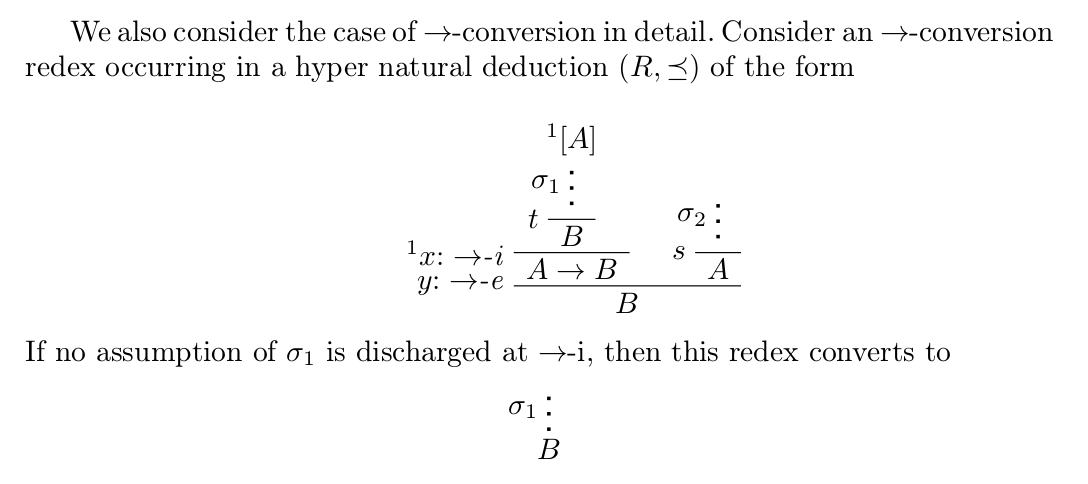
\includegraphics[width=\textwidth]{logic-example.png}

  20+ 年間:オーストリア(ウィーン工科大学)、イタリア(シエナ大学)、
  日本(北陸先端科学技術大学院大学)
\end{frame}

\begin{frame}[plain]
  \frametitle{Debian Developer}
  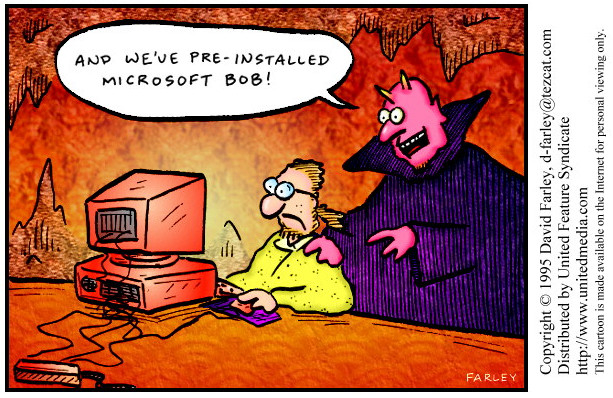
\includegraphics[width=\textwidth]{unixhell.png}

  だいたい\TeX 関係のパッケージ(プラスCalibre, mu, \ldots)
\end{frame}

\begin{frame}[plain]
  \frametitle{\TeX\ Live Developer}
  
\includegraphics[width=\textwidth]{texlive2018.png}

  \TeX\ Live (メーンインフラ開発者)、日本語サポート(\url{texjp.org})
\end{frame}

\begin{frame}[plain]
  \frametitle{国際山岳ガイド}
  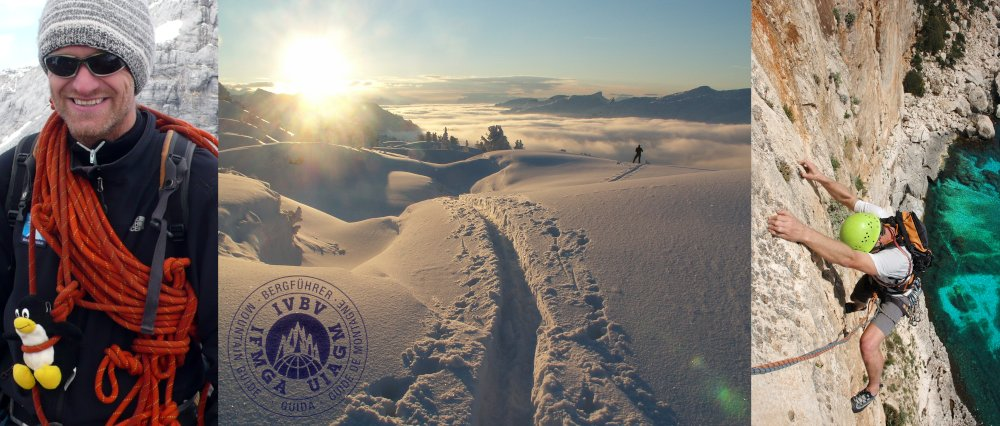
\includegraphics[width=\textwidth]{norbert-guide.jpg}

  岩登り、山スキー、アイスクライミング、ハイキング、沢登り、\ldots
\end{frame}

\begin{frame}[plain]
  \frametitle{アクセリア株式会社・研究開発部}
  CDN、ウェブサービス、セキュリティーなどのサービス\footnote{\url{http://www.accelia.net}}
  
  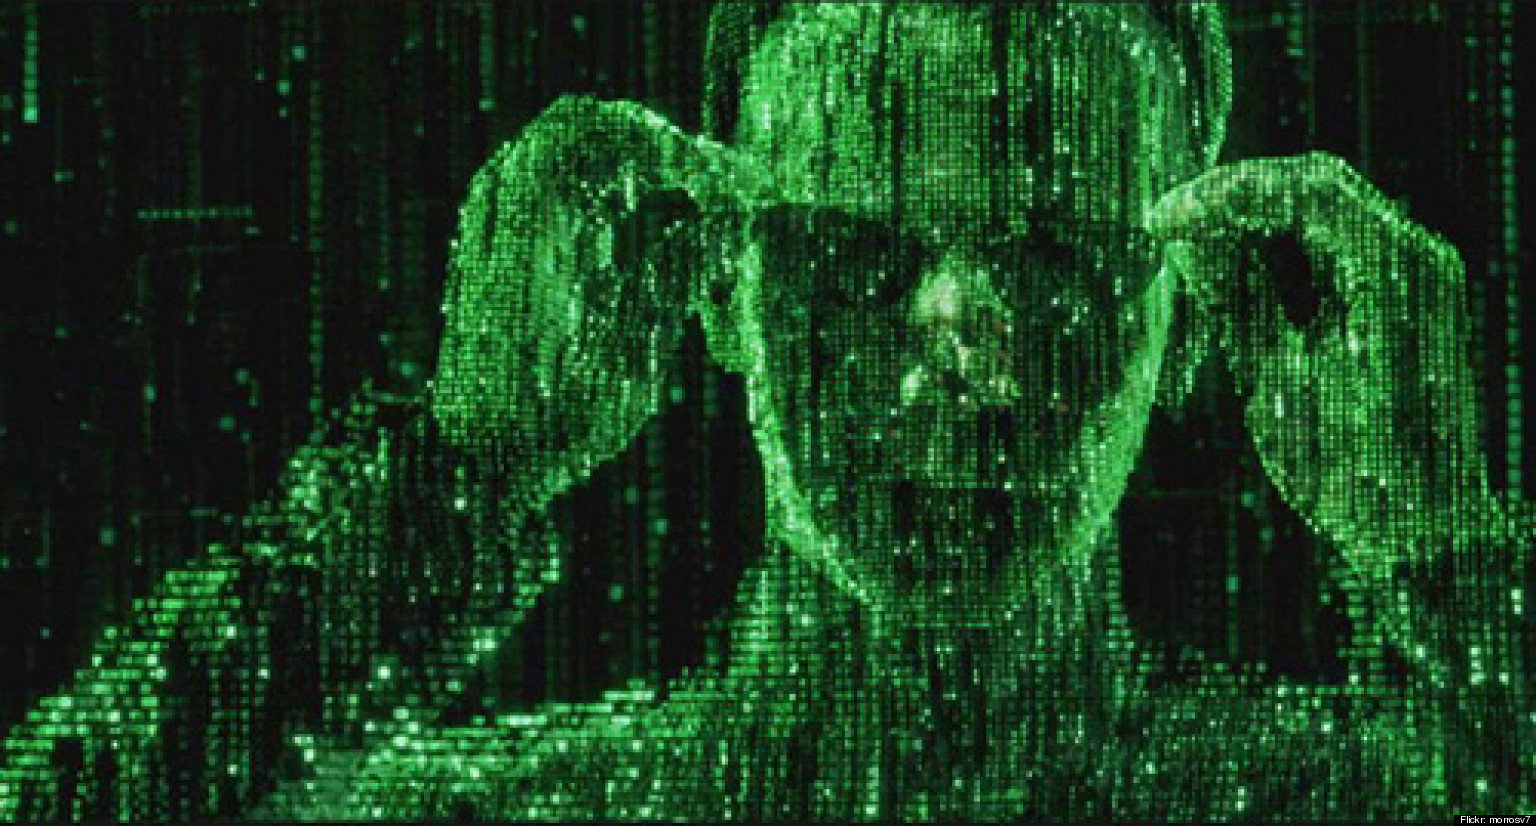
\includegraphics[width=\textwidth]{the-matrix.jpg}

  セキュリティー、機械学習、ソフトウェア検証、ブロックチェーン等
\end{frame}

\cutin{\tl\ とは何か?}

\begin{frame}
  \frametitle{\tl}
  \begin{itemize}
  \item \TeX とそのまわりのプログラム:
    pdftex, luatex, ptex, uptex, dvips, dvipdfmx, mf, xetex, detex,
    ht, patgen, \ldots\bis\pause
  \item \LaTeX\ macro and font package:\\
    memoir, beamer, lm, dejavu, fira, ipaex, libertine,
    \ldots\bis\pause
  \item \tlmgr: online update、 設定、検索など
  \end{itemize}
\end{frame}

\begin{frame}
  \frametitle{フィーチャー}

  \begin{itemize}
  \item `完成' -- 全ての\acro{CTAN}にあるOSSパッケージを含む
  \item マルチープラットフォーム、同じシステム\\
    Windows == Unix (\emph{cum grano salis})
  \item 毎日の更新
  \item \acro{DFSG} フリー
  \item 様々のインストール方法(\acro{DVD}, network, mirror of \ctan, 
	svn checkout, 他のインストール)
  \item インストーラー:テクストと\acro{GUI}モード
  \item 翻訳された(日本語が含まれてる)
  \end{itemize}
\end{frame}

\begin{frame}[fragile]
  \frametitle{TLの歴史}
  \begin{itemize}
  \item late 1993 Dutch \TeX\ Users Group, 4All\TeX\ CD, \acro{tds}
    working group\pause
  \item 1995 Unix-based \acro{TDS} \acro{CD} based on te\TeX\pause
  \item 1996 first edition, Sebastian Rahtz%
    \uncover<3-3>{\img{rahtz.png}{110pt}{10pt}{-5pt}}\pause
  \item 2000 5th edition, non-free software removed\pause
  \item 2002 7th edition: Mac OS X support\pause
  \item 2005 addition of the -sys scripts\pause
  \item 2006-09 Xe\TeX\ addition, end of te\TeX\ development, 
    \TeX{}works addition,
    Karl Berry
    \uncover<7-7>{\img{berry.jpg}{100pt}{40pt}{-130pt}}
    \pause
  \item 2010- incremental inclusion of Japanese \TeX\ support 
  \end{itemize}
\end{frame}

\begin{frame}
  \frametitle{インストーラーの設定}
  \begin{itemize}
  \item arch/osシステム
    \uncover<1-1>{\img{gui-systems.png}{\textheight}{20pt}{-60pt}}\bigit
    \pause
  \item schemes
    \uncover<2-2>{\img{gui-scheme}{180pt}{45pt}{-80pt}}\pause\bigit
  \item collections
    \uncover<3-3>{\img{gui-collections}{170pt}{20pt}{-100pt}}
  \end{itemize}
\end{frame}

\cutin{\tl のパッケージ組織}

\begin{frame}
  \frametitle{3つのレベル}
  \begin{itemize}
  \item Package:基本のユニット、\acro{CTAN}のパッケージはだいたい\tl
    のPackageになる\\
    beamer, memoir, pgf, \ldots\bis
  \item Collection:関係があるパッケージの集合\\
    collection-fontsrecommended, collection-mathscience, \ldots\bis
  \item Schema:トップレベル、collectionとpackageを含む\\
    scheme-basic, scheme-standard, scheme-full, \ldots
  \end{itemize}

  「含む」はdependsという関係がある
\end{frame}

\begin{frame}[fragile,plain]
  \frametitle{\tl データベース:Package}
\begin{lstlisting}
name 12many
category Package
revision 15878
catalogue one2many
shortdesc Generalising mathematical index sets
longdesc In the discrete branches of mathematics and the computer
..
docfiles size=98
 texmf-dist/doc/latex/12many/12many.pdf details="Package documentation"
 texmf-dist/doc/latex/12many/README details="Readme"
srcfiles size=6
 texmf-dist/source/latex/12many/12many.dtx
 texmf-dist/source/latex/12many/12many.ins
runfiles size=1
 texmf-dist/tex/latex/12many/12many.sty
..
\end{lstlisting}
\end{frame}

\begin{frame}[fragile,plain]
  \frametitle{\tl データベース:Collection}
\begin{lstlisting}
name collection-langjapanese
category Collection
revision 48752
shortdesc Japanese
longdesc Support for Japanese; additional packages in
longdesc collection-langcjk.
depend collection-langcjk
depend ascmac
depend babel-japanese
depend bxbase
depend bxcjkjatype
depend bxjalipsum
depend bxjaprnind
depend bxjscls
depend bxorigcapt
..
\end{lstlisting}
\end{frame}

\begin{frame}[fragile,plain]
  \frametitle{\tl データベース:Schema}
\begin{lstlisting}
name scheme-medium
category Scheme
revision 44177
shortdesc medium scheme (small + more packages and languages)
longdesc This is the medium TeX Live collection: it contains plain TeX,
longdesc LaTeX, many recommended packages, and support for most European
longdesc languages.
depend collection-basic
depend collection-binextra
depend collection-context
depend collection-fontsrecommended
depend collection-fontutils
depend collection-langczechslovak
depend collection-langenglish
depend collection-langeuropean
..
\end{lstlisting}
\end{frame}


\begin{frame}
  \frametitle{数・数・数}
  現在の\tl に含まれてるのは:
  \begin{itemize}
  \item 9 Scheme\bis
  \item 41 Collection\bis
  \item 6718 Package\bis
  \item 181839 Files\bis
  \item 17 architecture-os combinations
  \end{itemize}
\end{frame}

\cutin{Neo4jへ}

\begin{frame}
  \frametitle{\tl\ DatabaseからNeo4jへ}
  \begin{itemize}
  \item 簡単なPerlスクリプト\bis
  \item \tl のPerl Modulesを使う\bis
  \item CSVにエクスポート\bis
  \item neo4j-importでインポート
  \end{itemize}
\end{frame}

\begin{frame}[fragile]
  \frametitle{CSV: node-Package.csv}
  \begin{lstlisting}
uuid:ID,name
idde511a2208a14810b27f36ddbb0065a8,mkpic
ida7ce0776c7f64cefa2e2a74bd94268a1,mpcolornames
idc63eeda473104ebea21e5844dd7c5660,gfnotation
id3cfc0196bf5c4c1baeffabca67b9a544,turkmen
id3b602a6c491544deb2edd510c1fe2c20,cascadilla
...
\end{lstlisting}

\end{frame}


\begin{frame}[fragile]
  \frametitle{CSV: node-Collection.csv}
  \begin{lstlisting}
uuid:ID,name
id96c30fc211be44219457852dc835fd2a,collection-langczechslovak
ide1788d667112443b9fe1eba27628498c,collection-langcyrillic
id186afd7ec58e4285a09dbfe7650f6542,collection-langjapanese
id100a6c30d11d443191ba4abab9be9d37,collection-wintools
id00b2ac0c815b48eb866029f530c525ad,collection-pictures
...
\end{lstlisting}

\end{frame}



\begin{frame}[fragile]
  \frametitle{CSV: edge-depends.csv}
  \begin{lstlisting}
:START_ID,:END_ID
idc9215c5d96bf4cb587785d8c0d50a6e0,id120a994a30204e40bf158b76f6eb9e87
idc9215c5d96bf4cb587785d8c0d50a6e0,idf989960c4f494e1a90f09adcfbf25d31
id96c30fc211be44219457852dc835fd2a,id2883c1628d4544cc8e461dbf2e88a42d
id96c30fc211be44219457852dc835fd2a,id10536fb246e9471d86e36ff7200e77d9
id96c30fc211be44219457852dc835fd2a,idc3e0c0d5add747e39ffd9ab95fed3920
...
\end{lstlisting}

\end{frame}


\begin{frame}[fragile]
  \frametitle{CSV: edge-contains.csv}
  どのファイルはどのパッケージに含まれてる情報
  \begin{lstlisting}
:START_ID,type,:END_ID
id0ecf144c7bfc4c7a8037981121810d8d,doc,id82f6f55fe13d4e74b42f884c7a1d1dc8
idf4166223dcdb446b95ac9d9e551ea562,run,ideba9104946c64d48b0849c1361d94dcc
id6d704e156bed47d39f41ebd1ce447dae,run,id6616c86a71854f718b964cade207e4bf
id6e0b59327a5942b49aa670f815f4a579,run,idee5780bcadb04ab2b678b2fc56594b85
id469eb48326ce46e7a213d52fddfcc91a,doc,ide535515a72314cb589cdfa622d73b6f6
...
\end{lstlisting}

\end{frame}

\begin{frame}[fragile,plain]
  %\frametitle{Neo4jへのインポート}
\begin{lstlisting}
$ ls
edge-contains.csv    node-ConTeXt.csv  node-Scheme.csv
edge-depends.csv     node-Files.csv    node-TLCore.csv
node-Collection.csv  node-Package.csv
$ neo4j-import --into ../graphdb \
--nodes:Collection node-Collection.csv \
--nodes:ConTeXt node-ConTeXt.csv \
--nodes:Files node-Files.csv \
--nodes:Package node-Package.csv \
--nodes:Scheme node-Scheme.csv \
--nodes:TLCore node-TLCore.csv \
--relationships:contains edge-contains.csv \
--relationships:depends edge-depends.csv
...
IMPORT DONE in 4s 199ms. 
Imported:
  168140 nodes
  168803 relationships
  336280 properties
Peak memory usage: 1.03 GB
\end{lstlisting}
\end{frame}
\cutin{パッケージグラフでの模索}

\begin{frame}[fragile]
  \frametitle{簡単なCypherでの模索}
  \pause
  全てのSchema
  \begin{lstlisting}
match (s:Scheme) return s;   
\end{lstlisting}

\pause
Collection以外のSchemaの依存
\begin{lstlisting}
match p = (s:Scheme) -[:depends]-> (q)
  where NOT 'Collection' IN LABELS(q)
  return p;
\end{lstlisting}
\end{frame}

\begin{frame}[fragile]
  \frametitle{一貫性の確認}
  \pause
  複数のCollectionに入ってるパッケージがない
\begin{lstlisting}
match (c1:Collection) -[:depends]-> (p)
  <-[:depends]- (c2:Collection) return c1, c2, p;
\end{lstlisting}
\pause
サイクルがない
\begin{lstlisting}
match p = (n)-[:depends*]-> (n) return p;
\end{lstlisting}

\pause
複数のパッケージに入ってるファイルがない
\begin{lstlisting}
match (p1) -[:contains]-> (f)
  <- [:contains]- (p2) return p1, p2, f;
\end{lstlisting}

\end{frame}


\begin{frame}[fragile]
  \frametitle{ファイルタイプの検索}
  1つのパッケージの全てのドキュメンテーションファイルの検索
\begin{lstlisting}
match (p) -[:contains {type:'doc'}]-> (f)
  where p.name = "tlcockpit"
  return p,f;
\end{lstlisting}
  
\end{frame}

\cutin{グラフ・アルゴリズム}

\begin{frame}
  \frametitle{グラフ・アルゴリズムライブラリのインストール}
  \begin{itemize}
  \item \url{https://neo4j.com/docs/graph-algorithms/current/}
  \item \texttt{graph-algorithms-algo-3.4.7.0.jar}をNeo4jの
    \texttt{plugins}フォルダにおく
  \item Neo4jのconfig fileに\\
    \texttt{dbms.security.procedures.unrestricted=algo.*}\\
    を書き込む
  \item Neo4jを再起動
  \end{itemize}
\end{frame}

\begin{frame}[fragile]
  \frametitle{Google Page Rank}
\begin{lstlisting}
CALL algo.pageRank.stream(null, 'depends',
  {iterations:20, dampingFactor:0.85})
YIELD nodeId, score
MATCH (node) WHERE id(node) = nodeId
RETURN node.name AS page,score
ORDER BY score DESC
\end{lstlisting}
\end{frame}

\begin{frame}[fragile]
  \frametitle{Page rankの結果}
  \begin{tabular}{ll}
    \toprule
    page & score\\
    \midrule
context & 4.868265000000001\\
hyphen-base                 &4.667172000000001  \\
hyph-utf8                   &4.0754105          \\
kpathsea                    &1.8529665          \\
plain                       &0.982524           \\
cm                          &0.6986750000000002 \\
luatex                      &0.656277           \\
pdftex                      &0.621257           \\
    collection-basic            &0.556997           \\
    \bottomrule
  \end{tabular}
\end{frame}

\begin{frame}[fragile]
  \frametitle{Betweenness Centrality}
\begin{lstlisting}
CALL algo.betweenness.stream(null,'depends',
  {direction:'out'})
YIELD nodeId, centrality
MATCH (pkg) WHERE id(pkg) = nodeId
RETURN pkg.name AS pkg,centrality
ORDER BY centrality DESC;
\end{lstlisting}
\end{frame}

\begin{frame}
  \frametitle{Betweennessの結果}
  \begin{tabular}{ll}
    \toprule
    pkg &centrality \\
    \midrule
    collection-basic &1675.4717032967033\\
    collection-latexextra & 1212.0             \\
    context & 947.3333333333334  \\
    collection-latex & 744.8166666666666  \\
    collection-pictures & 586.0              \\
    collection-mathscience & 528.0              \\
    collection-plaingeneric & 448.5              \\
    collection-latexrecommended & 412.0              \\
    xetex & 336.41666666666663 \\
    \bottomrule
  \end{tabular}
\end{frame}


\begin{frame}[fragile]
  \frametitle{Triangle computation}
\begin{lstlisting}
CALL algo.triangleCount.stream(null, 'depends',
  {concurrency:4})
YIELD nodeId, triangles, coefficient
MATCH (p) WHERE id(p) = nodeId
RETURN p.name AS name, triangles, coefficient
ORDER BY triangles DESC
\end{lstlisting}
\end{frame}

\begin{frame}
  \frametitle{結論}
  \begin{itemize}
  \item Neo4jで簡単に任意のシステムを表現できる\bis\pause
  \item 簡単なCypherで複雑な状況を確認できる\bis\pause
  \item 早い(今日だけの準備!)\bis\pause
  \end{itemize}

  興味があれば
  \begin{center}
    \url{http://www.texlive.info:7474/}
  \end{center}
  で遊んでいい ;-) (read-only)

  \pause
  ありがとうございます
\end{frame}

\end{document}


%%% Local Variables:
%%% mode: latex
%%% TeX-engine: luatex
%%% TeX-master: t
%%% End:
